% !TEX encoding = UTF-8 Unicode
\documentclass[a4paper]{article}

\usepackage{color}
\usepackage{url}
\usepackage[T2A]{fontenc} % enable Cyrillic fonts
\usepackage[utf8]{inputenc} % make weird characters work
\usepackage{graphicx}
\usepackage{wrapfig}

\usepackage[english,serbian]{babel}
%\usepackage[english,serbianc]{babel} %ukljuciti babel sa ovim opcijama, umesto gornjim, ukoliko se koristi cirilica

\usepackage[unicode]{hyperref}
\hypersetup{colorlinks,citecolor=green,filecolor=green,linkcolor=blue,urlcolor=blue}

\usepackage{listings}

%\newtheorem{primer}{Пример}[section] %ćirilični primer
\usepackage{ntheorem}
\theoremstyle{break}
\newtheorem{primer}{Primer}[section]

\definecolor{mygreen}{rgb}{0,0.6,0}
\definecolor{mygray}{rgb}{0.5,0.5,0.5}
\definecolor{mymauve}{rgb}{0.58,0,0.82}

\lstset{ 
  backgroundcolor=\color{white},   % choose the background color; you must add \usepackage{color} or \usepackage{xcolor}; should come as last argument
  basicstyle=\footnotesize,        % the size of the fonts that are used for the code
  breakatwhitespace=false,         % sets if automatic breaks should only happen at whitespace
  breaklines=true,                 % sets automatic line breaking
  captionpos=b,                    % sets the caption-position to bottom
  commentstyle=\color{mygreen},    % comment style
  deletekeywords={...},            % if you want to delete keywords from the given language
  escapeinside={\%*}{*)},          % if you want to add LaTeX within your code
  extendedchars=true,              % lets you use non-ASCII characters; for 8-bits encodings only, does not work with UTF-8
  frame=single,	                   % adds a frame around the code
  keepspaces=true,                 % keeps spaces in text, useful for keeping indentation of code (possibly needs columns=flexible)
  keywordstyle=\color{blue},       % keyword style
  language=SQL,                 % the language of the code
  morekeywords={*,...},            % if you want to add more keywords to the set
  numbers=none,                    % where to put the line-numbers; possible values are (none, left, right)
  rulecolor=\color{black},         % if not set, the frame-color may be changed on line-breaks within not-black text (e.g. comments (green here))
  showspaces=false,                % show spaces everywhere adding particular underscores; it overrides 'showstringspaces'
  showstringspaces=false,          % underline spaces within strings only
  showtabs=false,                  % show tabs within strings adding particular underscores
  stepnumber=1,                    % the step between two line-numbers. If it's 1, each line will be numbered
  stringstyle=\color{mymauve},     % string literal style
  tabsize=2,	                     % sets default tabsize to 2 spaces
}

\begin{document}

\title{Da li ste bezbedni na Internetu?\\ \small{Seminarski rad u okviru kursa\\Metodologija stručnog i naučnog rada\\ Matematički fakultet}}

\author{Nevena Ajvaz, Natalija Jovanović, Marija Milićević, Tijana Nikčević\\ nevena.ajvaz@hotmail.com, natalija.jovanovic996@gmail.com,\\
marija.milicevic.10.23@gmail.com, tijana.nikcevic1@gmail.com}

\date{April 2019.}

\maketitle

\abstract{
Internet je jedno od najmoćnijih oružja današnjice koji nudi mnoge pogodnosti ako se koristi u prave svrhe. Bezbednost na Internetu je veoma veliki problem i u vezi sa tim upoznaćemo se sa najčešćim vrstama sajber napada, kriminala i pojmom glasanja putem Interneta. Videćemo zašto je naša bezbednost ugrožena i kroz primere poznatih napada opisati načine na koje se ona narušava.

\tableofcontents

\newpage

\section{Uvod}
\label{sec:uvod}

U ovom radu ćemo se na početku upoznati sa pojmom sajber kriminala\cite{kriminal}, kao i problemom rasprostranjenosti sajber napada. Dalje će biti prikazane 3 najčešće vrste napada - fišing, SQL injekcija \cite{sql_injection} i DoS. Sajber kriminal brzo napreduje, što prouzrokuje razvoj i nastanak novih vrsta napada. U petom poglavlju, koje se odnosi na primere napada, biće prikazani problemi najvećih svetskih kompanija \cite{kompanije} i država \cite{knjiga}, i kako su se one suočavale sa tim. Nakon ovoga, pozabavićemo se temom glasanja putem Interneta.


%Broj naslova i podnaslova je proizvoljan. Neophodni su samo Uvod i Zaključak. Na poglavlja unutar teksta referisati se po potrebi. 
%\begin{primer}
%U odeljku \ref{sec:naslov1} precizirani su osnovni pojmovi, dok su zaključci dati u odeljku \ref{sec:zakljucak}.
%\end{primer}

%Još jednom da napomenem da nema razloga da pišete:
%\begin{verbatim}
%\v{s} i \v{c} i \'c ...
%\end{verbatim}
%Možete koristiti srpska slova
%\begin{verbatim}
%š i č i ć ... 
%\end{verbatim}



%\section{Slike i tabele}
%\label{slike_i_tabele}

%Slike i tabele treba da budu u svom okruženju, sa odgovarajućim naslovima, obeležene labelom da koje omogućava referenciranje. 

%\begin{primer} Ovako se ubacuje slika. Obratiti pažnju da je dodato i 
%\begin{verbatim}
%\usepackage{graphicx}
%\end{verbatim}

%\begin{figure}[h!]
%\begin{center}
%\includegraphics[scale=0.75]{panda.jpg}
%\end{center}
%\caption{Pande}
%\label{fig:pande}
%\end{figure}

%Na svaku sliku neophodno je referisati se negde u tekstu. Na primer, na slici \ref{fig:pande} prikazane su pande. 
%\end{primer}

%\begin{primer} I tabele treba da budu u svom okruženju, i na njih je neophodno referisati se u tekstu. Na primer, u tabeli \ref{tab:tabela1} su prikazana različita poravnanja u tabelama.

%\begin{table}[h!]
%\begin{center}
%\caption{Razlčita poravnanja u okviru iste tabele ne treba koristiti jer su nepregledna.}
%\begin{tabular}{|c|l|r|} \hline
%centralno poravnanje& levo poravnanje& desno poravnanje\\ \hline
%a &b&c\\ \hline
%d &e&f\\ \hline
%\end{tabular}
%\label{tab:tabela1}
%\end{center}
%\end{table}

%\end{primer}

%\section{K\^{o}d i paket listings}
%Za ubacivanje koda koristite paket \textbf{listings}:
%\url{https://en.wikibooks.org/wiki/LaTeX/Source_Code_Listings}

%Primer ubacivanja koda
%\begin{lstlisting}[frame=single]
%# This program adds up integers in the command line
%import sys
%try:
%    total = sum(int(arg) for arg in sys.argv[1:])
%    print 'sum =', total
%except ValueError:
%    print 'Please supply integer arguments'
%\end{lstlisting}


\section{Pojam sajber kriminala}
\label{pojam}

Visokotehnološki ili sajber kriminal (eng. {\em cyber crime}) predstavlja moderni vid kriminala, tačnije, putem računara. Sajber kriminalci su osobe ili grupe ljudi koji koriste tehnologiju kako bi izveli zlonamerne aktivnosti putem mreže sa ciljem da ukradu osetljive podatke neke firme, lične informacije ili da profitiraju \cite{sajber}.
\\Zakoni koji se odnose na ovu vrstu kriminala se dopunjuju i razvijaju u zemljama širom sveta. Nerazvijene zemlje su najizloženije sajber napadima. U takvim zemljama je zakon o ovoj oblasti slabo definisan, a u nekim ni ne postoji. Takođe, veoma je teško pronaći i uhapsiti zločinca u sajber kriminalu jer su dokazi često nepostojeći.

Treba napraviti razliku između sajber kriminalca i hakera. Sajber kriminalci sa lošim namerama vrše upad u računare, dok hakeri traže inovativne načine da koriste sistem, bili ti načini loši ili dobri.
\\

 

\section{Vrste sajber napada}

\label{sec:vrste_sajber_napada}

U mnogim zemljama, Internet odvija ključnu ulogu u svakodnevnom životu ljudi. Olakšava virtuelnu komunikaciju među ljudima, podstiče razvoj novih poslovnih modela i kompanija, menja način na koji ljudi kupuju. U 2018. godini, transfer novca koji uključuje prodaju i kupovinu putem Interneta, iznosila je oko \$2.8 biliona. Prema statističkim studijama \cite{statistika}, smatra se da će u 2021. ta vrednost iznositi oko \$4.88 biliona. Iz ovih razloga, nije neobično da je sa porastom popularnosti Interneta porasla i stopa kriminala na njemu. U ovom poglavlju će biti obrađene tri vrste napada putem Interneta.

\subsection{Fišing (eng. {\em phishing})}
\label{subsec:phishing}

Fišing je vrsta društvenog inženjeringa (eng. {\em social engineering})\footnote{Obmana kojom se manipuliše ljudima da daju poverljive informacije.} gde se napadač pomoću elektronske pošte ili zlonamernih veb sajtova lažno predstavlja kao pouzdana organizacija ili kompanija kako bi prikupio lične podatke od pojedinca ili kompanije \cite{phishing_us_cert}. Engleski termin {\em  phishing} je prvi put koriščen 1996. a nazvan je po pecanju jer mejlovi služe kao mamac kojim se ljudi navode da daju svoje podatke. ,,Ph‘‘ umesto ,,f‘‘ u zapisu reči je aluzija na termin {\em phreaks} koji označava ljude koji su eksploatisali telekomunikacije, a neki ih smatraju i prvim hakerima \cite{phishing_org}.
Napadi fišinga se često sastoje od slanja korisnicima mejlova koji izgledaju kao da su iz bankarske ili finansijske institucije ili veb servisa preko kojeg pojedinac ima račun. Cilj fišinga je da prevari primaoca da da svoje podatke za prijavljivanje ili druge osetljive informacije. 
Na primer, napadač može da pošalje milione mejlova sa botnet-a\footnote{Mreža privatnih računara, zaraženih zlonamernim softverom, koji se kontrolišu kao grupa bez znanja vlasnika, npr. za slanje spama.}. Poruke obaveštavaju primaoce da je njihov nalog za elektronsku trgovinu bio kompromitovan i upućuju ih na veb lokaciju gde bi rešili problem. Korisnici koji kliknu na link dođu do veb stranice koja je napravljena tako da podseća na originalni sajt za elektronsku trgovinu. Kada se nađu na sajtu, od njih se traži korisničko ime, lozinka i druge privatne informacije. Te informacije mogu da se iskoriste za krađu identiteta. Jedni od glavnih načina zaštite od fišing napada su oprez i učenje kako se identifikuju sumnjivi imejlovi \cite{phishing_prevent}.

Ciljano orijentisan fišing (eng. {\em spear phishing}) je varijanta fišinga u kojoj napadač bira adrese elektonske pošte tako da cilja jednog ili određenu grupu primalaca. Na primer, napadač može ciljati starije osobe kao osobe koje se smatraju lakovernijima ili članove grupa koji imaju pristup vrednim informacijama. Ciljano orijentisan fišing može biti veoma delotvoran jer omogućava napadaču da uobliči napad tako da žrtva zbog hitnosti ili poverenja određenim osobama bude manje oprezna. Za ovo je potrebno da napadač prikupi lične podatke o žrtvi, kao što su imena prijatelja, poslodavac, rodni grad, lokacije koje posećuje, šta je nedavno kupila na mreži itd.
Na primer, napadač može da pošalje mejl ka nekoliko ljudi koji izgleda kao da je od njihovog direktora, kojim ih poziva na sastanak putem Gmail-a, a link u poruci navodi primaoce da se prijave na Gmail da prisustvuju sastanku. 

Fišing se pojavio negde oko 1995, ali je postao čest tek nakon 10 godina. Prvi napadi bili su vezani za AOL (eng. {\em America Online}), u to vreme najpopularniji internet provajder\cite {phishing_aol}. 2000ih godina su napadi prešli na platne sisteme poput E-Gold, eBay i PayPal.
Zanimljivo je povećanje napada na kinesku elektronsku trgovinu, što ukazuje na povećanje važnosti kineske ekonomije \cite{knjiga}.
Na slici \ref{fig:phishing_napadi} prikazana je količina sajtova za fišing koje je otkrila APWG (eng. {\em Anti-Phishing Working Group}) tokom godina \cite{apwg}.

\begin{figure}[h!]
\begin{center}
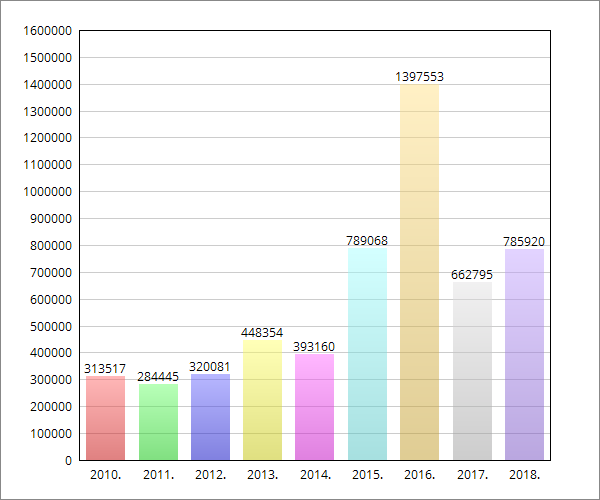
\includegraphics[width=0.48\textwidth]{phishing.png}
\end{center}
\caption{Količina otkrivenih sajtova za fišing}
\label{fig:phishing_napadi}
\end{figure}
\subsection{SQL injekcija}
\label{subsec:sql}

SQL\footnote{Standardni jezik za skladištenje, manipulaciju i dohvatanje podataka u bazama podataka.} injekcija je umetanje dela ili celog SQL upita obično preko polja za unos na veb stranici. Ukoliko ovako nešto uspe može se pristupiti osetljivim podacima iz baze, mogu se modifikovati podaci, izvršiti administrativne operacije nad bazom itd. 

\begin{primer}
\label{primer_1}
\begin{lstlisting}[frame=single]
txtUserId = getRequestString("UserId");
txtSQL = "SELECT * FROM Users WHERE UserId = " + txtUserId;
\end{lstlisting}
\end{primer}
\noindent U primeru \ref{primer_1} kreira se SELECT upit dodavanjem sadržaja promenljive txtUserId na select string. Sadržaj promenljive je sadržaj polja za unos korisničkog id-a.\\

Jedan od načina upotrebe SQL injekcije zasniva se na činjenici da je \texttt{1=1} uvek istinito. Pod pretpostavkom da je korisnik u polje za unos uneo \texttt{105 OR 1=1}, SQL upit iz primera \ref{primer_1} bi izgledao ovako:

\begin{lstlisting}[frame=single]
SELECT * FROM Users WHERE UserId = 105 OR 1=1;
\end{lstlisting}
\noindent Ovakav upit vratiće sve redove tabele ,,Users‘‘. Šta ako tabela ,,Users‘‘ sadrži imena i šifre? Može se pristupiti svim imenima i šiframa iz baze jednostavno dodavajući \texttt{105 OR 1=1} u polje za unos korisničkog imena.\\

\texttt{"}\texttt{"}=\texttt{"}\texttt{"} je uvek istinito. Ovo je još jedan način upotrebe SQL injekcije.
\begin{primer}
\label{primer_2}
\begin{lstlisting}[frame=single]
uName = getRequestString("username");
uPass = getRequestString("userpassword");

sql = 'SELECT * FROM Users WHERE Name ="' + uName + '" AND Pass ="' + uPass + '"'
\end{lstlisting}
\end{primer}

\noindent Ukoliko naš kod izgleda kao u primeru \ref{primer_2} može se pristupiti korisničkim imenima i šiframa u bazi unoseći \texttt{"} OR \texttt{"}\texttt{"}=\texttt{"} u polje za šifru i u polje za korisničko ime. Kod na serveru će kreirati ispravan SQL upit:

\begin{lstlisting}[frame=single]
SELECT * FROM Users WHERE Name ="" OR ""="" AND Pass ="" OR ""="";
\end{lstlisting}
\noindent Ovakav upit vratiće sve redove iz tabele ,,Users‘‘. 

Mnoge baze podržavaju grupu SQL upita razdvojenih ; simbolom. Ukoliko bi korisnik u polje za korisnički id uneo \texttt{105; DROP TABLE Suppliers}, SQL upit iz primera \ref{primer_1} izgledao bi ovako:

\begin{lstlisting}[frame=single]
SELECT * FROM Users WHERE UserId = 105; DROP TABLE Suppliers; 
\end{lstlisting}
\paragraph{}
Zaštita od ovakvih napada je moguća korišćenjem SQL parametara. To su vredosti koje su dodate SQL upitu u vreme izvršavanja na kontrolisan način.

\begin{primer}
\label{primer_3}
\begin{lstlisting}[frame=single]
txtUserId = getRequestString("UserId");
txtSQL = "SELECT * FROM Users WHERE UserId = @0";
db.Execute(txtSQL,txtUserId);
\end{lstlisting}
\end{primer}
\noindent Primer \ref{primer_3} je deo koda u ASP.NET-u u kome se koriste parametri. Parametri su predstavljeni znakom @. SQL mehanizam proverava parametre kako bi se uverio da su ispravni i da se tretiraju bukvalno a ne kao deo SQL-a koji se izvršava.

\subsection{DoS napadi}
\label{subsec:DoS}

DoS (eng. {\em Denial-of-Service}) napad je radnja koja sprečava legitimitne korisnike da koriste usluge računara, tj. napadač utiče da mašina ili mrežni resurs  budu nedostupni korisnicima tako što privremeno ili neograničeno ometa usluge hosta\footnote{Računar koji čuva veb sajt ili druge podatke kojima se može pristupiti preko Interneta ili neke druge mreže (izvor - \href{https://en.oxforddictionaries.com/definition/host}{Oxford Dictionaries}).} povezanog na Internet. DoS napad može da uključi neovlašćeni pristup jednom ili više računarskih sistema, ali cilj napada nije krađa informacija, nego remećenje sposobnosti servera da odgovori na korisničke zahteve tako što zatrpava metu mrežnim saobraćajem ili šalje informacije koje aktiviraju razne nezgode. Ometanje normalnog rada računarskih usluga može da napravi veliku štetu. Firma koja se bavi nekom vrstom prodaje putem Interneta može da izgubi posao, vojsci može da se prekine komunikacija, Vladi ili nekoj neprofitnoj organizaciji može da se desi da ne može da prenese svoju poruku javnosti.

DoS napad je primer ,,asimetričnog‘‘ napada, tj. napada u kome jedna osoba može dosta da naškodi velikoj organizaciji. Pošto se terorističke organizacije specijalizuju za asimetrične napade, neki strahuju da će DoS napadi postati važan deo terorističkog oružja.

\subsubsection{DDoS napadi}
\label{subsubsec:DDoS}

Dodatni tip DoS napada je DDoS (eng. {\em Distributed Denial-of-Service}) napad. Glavna razlika je u tome što meta nije napadnuta sa jedne lokacije, već sa više njih odjednom \cite{ddos}. Do DDoS napada se dolazi kada višestruki sistemi vode sinhronizovani DoS napad na jednu metu. Podela hostova koji određuju DDoS daje napadaču više prednosti:
\begin{itemize}
\item Napadač može iskoristiti veći kapacitet resursa mašine kako bi izvršio ozbiljan razoran napad
\item Lokacije napada se teško određuju zbog slučajne podele napadačkih sistema
\item Teže je ugasiti više mašina nego jednu
\item Pravu napadačku grupu (eng. {\em attacking party}) je veoma teško identifikovati, jer se oni prikrivaju iza mnogih (uglavnom kompromitovanih) sistema
\end{itemize}

Mnoge sigurnosne tehnologije su razvile mehanizme za odbranu od mnogih vrsta DoS napada, ali, zbog jedinstvenih karakteristika, DDoS se još uvek smatra ozbiljnom pretnjom.

\section{Sajber kriminal}
\label{sec:sajber_kriminal}

%http://docshare04.docshare.tips/files/23471/234718626.pdf \\

Glavni trend koji pokreće evoluciju računarskih napada i eksploatacija uključuje motiv rasta profita zasnovanog na zlonamernom kodu - malveru (eng. {\em malware, malicious code}). Neki napadači prodaju prilagođeni malver za kontrolu mašina žrtava kupcu koji je najviše ponudio. Mogu iznajmiti gomile zaraženih sistema, koji su korisni za isporuku nepoželjne pošte (spamova), fišing shema, DoS napada ili za krađu identiteta. Špijunske kompanije i preterano agresivni oglašivači kupuju takvu vrstu koda kako bi se infiltrirali i kontrolisali žrtvine mašine. Jedna zaražena mašina na kojoj iskaču reklame i prilagođavaju se rezultati pretrage može da košta svega \$1 mesečno. {\em Keylogger}\footnote{Softver ili hardver koji ima sposobnost da beleži sve što je otkucano na tastaturi i taj sadržaj čuva u kriptovanom fajlu.} na zaraženoj mašini može da pomogne napadaču da skupi brojeve kreditnih kartica i ukrade \$1000 ili više od žrtve pre nego što se otkrije prevara. Ako kontroliše 10000 mašina, napadač može solidno da zaradi od sajber kriminala. 
%Organizovane kriminalne grupe mogu okupiti grupu takvih napadača kako bi stvorile biznis, što izaziva porast industrije malvera. Krajem devedesetih godina prošlog veka, većinu malvera su pravili entuzijasti, ali danas su profesionalni napadači stavili cenu na svoj malver. 
%Njihovi profitni centri daju sredstva koja se mogu koristiti za istraživanje i razvoj kako bi se stvorio snažan zlonameran softver i ometali poslovni modeli, kao i finansirali drugi zločini. 

Kada kriminalci budu otkrili pouzdan način za zaradu novca na ovoj grani kriminala, broj incidenata ovog tipa će se neizbežno povećati. Napadači su osmislili različite poslovne modele koji su niskog rizika, tako da je mala verovatnoća da će napadač biti uhvaćen ukoliko pažljivo skriva svoje tragove. Tako mogu da se zarade stotine hiljada ili čak milioni dolara.

Faktor koji podstiče rast sajber napada je bot (skraćenica od reči \textit{robot}) softver. Ovaj softver dozvoljava napadaču da kontroliše neki sistem širom Interneta. Jedan napadač ili grupa napadača može da postavi ogromne botnet-ove širom sveta. Mašine koje kontrolišu botovi omogućavaju napadačima da postavljaju virtualne superračunare koji mogu da predstavljaju rivale nacionalnoj računarskoj snazi. Mogu da koriste te resurse da bi stvorili ogromnu poplavu, razbiju (eng. {\em crack}) kripto ključeve ili lozinke, ili da bi istražili osetljive finansijske podatke koji se koriste za krađu identiteta.

Botovi i ostali alati koji se koriste za napade su postali veoma modularni, svaki modul se sastoji iz softverskih komponenti koje omogućavaju napadačima da brzo menjaju funkcionalnost kako bi pokrenuli nove vrste napada. Obični botovi danas sadrže 50 do 100 različitih funkcionalnih modula; napadač može da ugasi ili odstrani module koji nisu potrebni za dati napad, dok lako integriše nove funkcije koda. 
%Drugi modularni napadački alati sadrže eksploatacione okvire (eng. {\em exploitation  frameworks}) koji prave pakovani eksploatacioni kod koji može da se infiltrira u ciljnu mašinu koja je ranjiva (zato što je pogrešno konfigurisana ili nepovezana).

Ubrzavajući evoluciju, napadači se sve više oslanjaju na bot kod koji se sam preobražava, dinamički stvarajući funkcionalno ekvivalentnu verziju sa različitim skupovima osnovnog koda. Takav polimorfni kod pomaže napadačima da izbegnu alate za detekciju koje antivirusi i \textit{antispyware} softveri\footnote{Vrsta programa napravljena za sprečavanje i otkrivanje neželjenih instalacija špijunskih softvera i uklanjanje tih programa ukoliko su instalirani.} danas koriste. Ovaj dinamički samopodešavajući kod je teže filtrirati, s obzirom da konstantno menja svoj osnovi softver. Ova ,,pokretna meta‘‘ koda otežava analizu od strane branilaca. Polimorfni kod podstiče ciljeve napadača jer napadači imaju dužu kontrolu nad botnetom izbegavajući filtriranje i detekcije, tako da mogu da zarade što više novca od zaraženih sistema.

\section{Sajber napadi}
\label{sec:sajber_napadi}

Sajber napad predstavlja napad od računara do računara koji povređuje poverljivost, integritet i informacije koje se nalaze na napadnutom računaru \cite{knjiga}. Na slici \ref{fig:primer_napada} se može videti kako proces jednog sajber napada može da izgleda. U ovom poglavlju ćemo se susresti sa nekim primerima napada na države i velike svetske gigante u poslednjih deset godina.

%\clearpage

\begin{figure}[h!]
\begin{center}
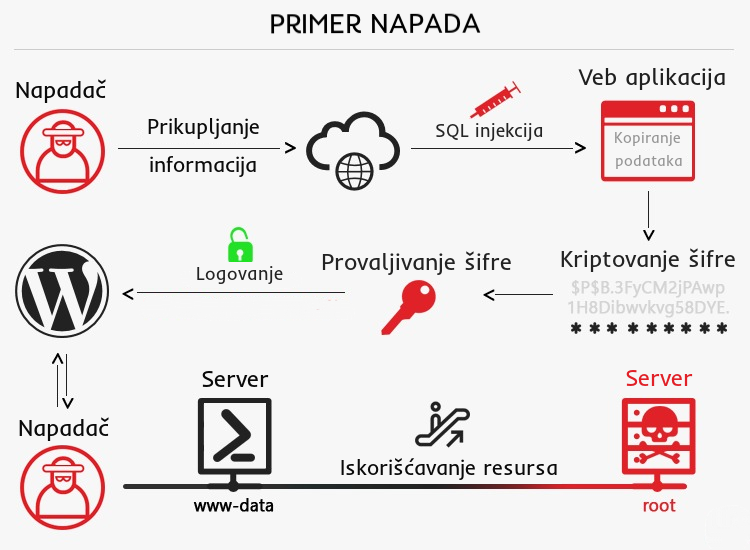
\includegraphics[width=0.48\textwidth]{napad.png}
\end{center}
\caption{Sajber napad}
\label{fig:primer_napada}
\end{figure}

\subsection{Primeri samostalnih napada}
\label{subsec:primeri_samo_napada}

\begin{description}
\item[DŽENSON DŽEJMS ANČETA] Dženson Džejms Ančeta, radnik u jednom Internet kafeu, je 2004. i 2005. napravio mrežu od oko 400000 botova, uključujući i računare kojima je upravljalo Ministarstvo odbrane SAD-a. Softveri za reklame (eng. {\em adware companies}), spameri i ostali su platili Ančeti da koriste te računare. Nakon što ga je FBI uhapsio, Ančeta se izjasnio krivim za razne optužbe, uključujući prekršavanje zakona o zlostavljanju računara. U maju 2005, federalni sudija je osudio Ančetu na 57 meseci zatvora i tražio od njega da plati \$15000 američkoj Vladi zbog napada na Ministarstvo odbrane. Zbog njegovih ilegalinih aktivnosti, Vlada je Ančeti oduzela njegov 1993 BMW, više od \$60000 u kešu, kao i njegovu računarsku opremu.


\item[PHARMAMASTER] Izraelska kompanija Blue Security je napravila sistem za zastrašivanje spamova kako bi pomogla ljudima koji ne žele da primaju spamove. Blue Security je prodavala svoj sistem preduzećima, dok su individualci mogli besplatno da štite svoje računare. Oko pola miliona ljudi se prijavilo za ovu besplatnu uslugu. Korisnici su na svojim računarima učitali bot po nazivu Blue Frog koji je integrisan sa Yahoo! Mail-om, Gmail-om, Hotmail-om i proverava da li su dolazeći mejlovi spamovi. Kada naiđe na spam poruku, bot kontaktira Blue Security server kako bi otkrio izvor tog mejla i zatim spameru šalje opt-out\footnote{Instrukcija od strane primaoca mejla da se spreči dalje slanje robe, informacija ili poruka od strane pojedinca ili kompanije.} poruku.

Spameri koji neselektivno šalju mejlove na milione adresa su počeli da primaju stotine hiljada opt-out poruka, koje su ometale njihove operacije. Šest najboljih svetskih spamera se dogovorilo da koristi softver za filtriranje koji je razvio Blue Security kako bi odstranili Blue Frog korisnike sa svojih mejl lista.

Jedan spamer, čiji je nadimak bio PharmaMaster, nije se povukao. On je pretio Blue Frog korisnicima porukama kao što je na primer sledeća: ,,Nažalost, zbog taktika koje koristi Blue Security, primaćete ovu poruku ili druge besmislene spamove 20-40 puta više nego inače‘‘. On je održao svoje obećanje, pa je 1. maja 2006. počeo da šalje Blue Frog korisnicima 10 do 20 puta više spamova nego inače.

Narednog dana je počeo da napada sam Blue Security. Lansirao je DDoS napad sa desetina hiljada botova ciljajući Blue Security servere. Ogromna količina dolaznih poruka je onemogućila Blue Frog uslugu. Kasnije su se DDoS napadi fokusirali na druge kompanije koje pružaju Internet usluge Blue Security-u. Na kraju su napadi ciljali preduzeća koja su plaćala usluge Blue Seciruty-u. Kada je Blue Security shvatio da ne može da zaštiti svoje klijente od DDoS napada i mejlova sa virusima, nevoljno je prekinuo svoju uslugu.

%\item[AVALANCHE GANG] Avalanche Gang je ime dato kriminalnom preduzeću koje je odgovorno za više fišing napada nego bilo koja druga organizacija. APWG\cite{apwg} je procenila da je Avalanche Gang odgovoran za dve trećine svih phishing napada lansiranih u drugoj polovini 2009. U drugoj polovini 2010, APWG je zapazila da je Avalanche skoro prestao sa fišing napadima, vodeći APWG da spekuliše da je Avalanche menjao strategije i fokusirao se na širenje neželjene pošte koja ljude uvlači u preuzimanje Zeus trojanca.


\item[ALBERT GONZALEZ] Albert Gonzalez je 2010. osuđen na 20 godina zatvora nakon što se izjasnio krivim za korišćenje SQL injekcija kako bi ukrao više od 130 miliona brojeva kreditnih i debitnih kartica. Neki od tih brojeva su prodati onlajn, što je dovelo do neovlašćenih kupovina i povlačenja banaka. Ciljevi napada su bili Heartland Payment Systems,  7-Eleven,  Hannaford Brothers Supermarkets,  TJX,  DSW,  Barnes \& Noble, OfficeMax, i Dave \& Buster lanci restorana. Većina brojeva je ukradena od firme Heartland Payment Systems, procenjujući gubitak na \$130 miliona.
\end{description}

\subsection{Primeri napada na države}
\label{subsec:primeri_napada_drzave}

\begin{description}
\item [GRUZIJA (2008)] Gruzija je jedna od bivših Sovjetskih republika koja je stekla nezavisnost 1991. godine. Južna Osetija, oblast na teritoriji Gruzije koja je pripadala Rusiji do 1991, nakon kratkog rata iste godine, postaje i međunarodno priznata kao autonomna pokrajina Gruzije. Nakon provokacije separatista u Južnoj Osetiji, Gruzija šalje vojsku na ovu teritoriju 7. avgusta 2008. godine. Ruske snage su 8. avgusta ušle u Južnu Osetiju i ove dve strane su se borile četiri dana. Ovaj sukob je ostao zapamćen i iz razloga što je gruzijska Vlada i pre nego što je ruska vojska došla na teritoriju Južne Osetije imala problem sa velikim DDoS napadom. Njihova Vlada nije bila u mogućnosti da komunicira sa ostatkom sveta. Mnogi veb sajtovi su bili srušeni na nekoliko sati. Gruzijska vlast je bila primorana da lokacije nekih svojih veb servera prebaci na SAD. Postojale su sumnje je da je napad izvršila grupa kriminalaca pod nazivom ,,Russian Business Network‘‘, smeštenih u Sankt Peterburgu u Rusiji, ali je ostalo nerazlučeno da li je ova grupa imala neke veze sa ruskom vojskom.
\\Na isti dan godinu dana kasnije, kompanija Twitter je bio onesposobljena u celom svetu na nekoliko sati zbog masovnih DDoS napada. Maks Keli, šef za bezbednost u kompaniji Facobook, rekao je da je svrha napada bila da se spreči objavljivanje teksta gruzijskog političkog blogera, pozivajući se na činjenicu da su istovremeno pali i ostali sajtovi koje je ovaj bloger koristio. Ti sajtovi su bili Facebook, LiveJournal i Google.     
\item [SAD I JUŽNA KOREJA (2009)] DDoS napad na američku i \linebreak južnokorejsku Vladu je izvršen tokom vikenda uoči 4. jula, američkog Dana nezavisnosti. Tom prilikom zabeležen je pad više od trećine veb sajtova u ovim državama. U Americi je napadnuta Bela kuća, američki trezor, Tajna služba, njujorška berza i kompanija NASDAQ. U Južnoj Koreji, DDoS napad je izvršen na Plavu kuću (predsednička palata), Ministarstvo odbrane i Narodnu skupštinu.
\\Ova vrsta napada se smatra relativno malom jer je izvršen uz pomoć botnet-a koristeći između 50 i 65 hiljada računara, što se smatra malom cifrom u poređenju na velike napade gde se koristi oko milion računara. Ipak, ova vrsta napada je ostala zapamćena i po tome što su južnokorejski sajtovi ostali nedostupni čak do 9. jula. Pretpostavljalo se da je napad izvršen kao vid osvete jer su Ujedinjene Nacije uvele određene sankcije Severnoj Koreji u tom periodu. I do danas se još uvek ne zna ko je tačno izveo ovaj napad jer su napadači koristili računare koji su bili u posedstvu drugih ljudi.    

\end{description}


\subsection{Primeri napada na kompanije}
\label{subsec:primeri_napada_kompanije}


\begin{description}
\item [Yahoo!] Yahoo! je jedan od najvećih giganta na Internetu. Ova kompanija je 2016. godine objavila informaciju da je bila žrtva jednog od najvećih napada u istoriji; 2013. je grupa hakera kompromitovala 3 milijarde naloga korisnika. Pored imena, datuma rođenja, mejl adresa i šifara, zaštitna pitanja i odgvori su takođe otkriveni. 
Pored ovog napada, 2014. je zabeležen još jedan napad na ovu kompaniju. Tada su obelodanjena imena, mejl adrese, datumi rođenja i brojevi telefona 500 miliona korisnika. Ovoga puta su šifre ostale zaštićene. 
\item [eBay] Ova kompanija se bavi prodajom proizvoda putem Interneta. Bila je napadnuta u maju 2014. kada su otkrivena imena, adrese, datumi rođenja i enkriptovane šifre\footnote{Ovakvi podaci su nečitljivi osobama koji ne poseduju ključ kako bi ih dekodirali i saznali njihovo značenje.} od 145 miliona korisnika. Kriminalci su ,,upali‘‘ u bazu tako što su koristili kreditacije troje zaposlenih i imali su pristup unutrašnjosti 229 dana. U tom periodu su imali vremena da pristupe bazi podataka korisnika. Informacije koje se tiču finansija kao što su brojevi kreditnih kartica su ostale zaštićene jer se ta vrsta podataka čuva u odvojenoj bazi.
\item [Uber] Uber je američka kompanija koja se predstavlja kao mreža koja pruža usluge transporta. Ona je 2016. bila napadnuta od strane samo dva hakera koji su uspeli da dođu do imena, mejl adresa i brojeva telefona 57 miliona korisnika Uber aplikacije. Takođe, otkriveni brojevi vozačkih dozvola 600 hiljada vozača na ovoj platformi.\\Hakeri su pristupili i Uberovom nalogu na GitHub platformi\footnote{Hosting servis baziran na vebu koji se koristi za kontrolu verzija. \url{https://github.com/}} gde su pronašli korisničko ime i lozinku kreditacije ka AWS\footnote{Amazon Web Services (AWS) je ogranak kompanije Amazon koja na zahtev pojedinca, kompanije ili Vlade pruža računarske resurse.} nalogu. 
Uber je ovaj napad objavio godinu dana kasnije. Ova kompanija je platila \$100 hiljada hakerima da unište podatke.  
\end{description}


\section{Glasanje putem Interneta}
\label{sec:glasanje}

Postoje mnogi načini na koje napadači mogu da naruše bezbednost umreženih računara. Međutim, praktičnost i niska cena obavljanja poslova putem Interneta donose značajne prednosti, pa nije iznenađujuće da se onlajn rešenje često predlaže kada postoji problem sa tradicionalnim načinom. U ovom delu biće prikazani predlozi za sprovođenje izbora putem Interneta.

\subsection{Motivacija za glasanje putem Interneta}
\label{subsec:Motivacija za glasanje putem Interneta}

Predsednički izbori 2000. godine su bili jedni od najneizvesnijih u istoriji SAD. Presudni su bili izborni glasovi države Florida. Bez njih ni demokrata Al Gor (eng. {\em Al Gore}), ni republikanac Džordž Buš (eng. {\em George V. Bush}) nisu imali većinu glasova. Buš je pobedio sa razlikom od 537 glasova u odnosu na Al Gora. Bušova prednost bila je neverovatno mala: manje od 2 glasa na svakih 10.000 glasova.

Većina okruga u Floridi koristila je mašinu za glasanje u kojoj birači biraju kandidata tako što olovkom probuše rupu u kartici pored odgovarajućeg imena (Slika \ref{fig:butterfly_ballot}). Prvi problem sa ovim načinom glasanja je da olovka ponekad ne probuši glatko rupu i takve glasove mašina za automatsko prebrojavanje obično ne uračuna. Zbog toga je bilo potrebno ručno prebrojavanje koje se fokusiralo na identifikaciji takvih glasačkih listića. Druga nepravilnost bila je da su neki birači u okrugu Palm Beach bili zbunjeni glasačkim listićima i želeći da glasaju za kandidata Al Gor koji je bio drugi na listi s leve strane, probušili drugu rupu koja zapravo odgovara kandidatu Patu Bakananu. Ova konfuzija je možda koštala Al Gora glasova koji su mu bili potrebni za pobedu na Floridi.
\begin{figure}[h!]
\begin{center}
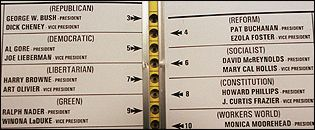
\includegraphics[width=0.6\textwidth]{butterfly_ballot.jpg}
%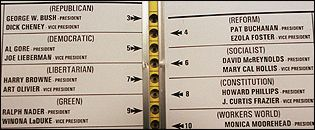
\includegraphics[scale=0.75]{butterfly_ballot.jpg}
\end{center}
\caption{Glasački listić - predsednički izbori na Floridi, SAD 2000.g.}
\label{fig:butterfly_ballot}
\end{figure}

Problemi sa izborima na Floridi doveli su do raznih akcija za poboljšanje pouzdanosti glasačkih sistema u SAD \cite{knjiga}. Mnoge države su zamenile papirne sisteme elektronskim glasačkim aparatima za direktno očitavanje, a neke su predložile da se koristi glasanje putem Interneta.
Međutim, glasanje putem Interneta u SAD je i danas omogućeno samo za vojna lica u inostranstvu i to samo u nekim državama \cite{i_voting}. Estonija je bila prva zemlja koja je omogućila svim svojim građanima da glasaju putem Interneta na lokalnim i nacionalnim izborima, 2005. godine. 
Norveška je omogućila glasanje putem Interneta 2011. i 2013. godine, ali se nakon toga vratila na stari način glasanja. Postoji 14 zemalja koje u današnje vreme koriste Internet kao opciju za glasanja, makar u nekim svojim delovima i tu spadaju i Kanada, Francuska i Švajcarska.

\subsection{Etička procena}
\label{subsec:Eticka procena}

U ovom poglavlju biće diskutovano o glasanju putem Interneta na osnovu prikazanih rizika i benefita.\\

\noindent BENEFITI GLASANJA PUTEM INTERNETA
\begin{itemize}
\item Glasanje putem Interneta daje ljudima priliku da glasaju iz svojh domova, ukoliko nisu u mogućnosti da dođu do biračkog mesta.
\item Glasovi koji se šalju putem Interneta mogu se prebrojati mnogo brže od glasova na papiru.
\item Elektronski glasovi ne bi imali nikakvu dvosmislenost.
\item Izbori koji su sprovedeni na Internetu koštali bi manje nego tradicionalni izbori.
\item Glasanje putem Interneta eliminisalo bi rizik da neko manipuliše glasačkom kutijom u kojoj se nalaze glasački listići.
\item Dok na većini izbora ljudi glasaju za jednog kandidata, drugi izbori omogućavaju da osoba glasa za više kandidata. Na primer, školski odbor može imati tri slobodna radna mesta, a od glasača se moze tražiti da glasaju za tri kandidata. Bilo bi lako isprogramirati obrazac za glasanje kako bi se sprečilo da ljudi glasaju za više ljudi nego što bi trebalo.
\item Ponekad, dugi i komplikovani glasački papiri rezultiraju tome da glasač slucajno zaboravi da zaokruži kandidata za određenu poziciju. Veb forma bi mogla da se dizajnira da bude na više strana i da svaka strana ima kandidata za jednu poziciju.
\end{itemize}


\noindent RIZICI GLASANJA PUTEM INTERNETA
\begin{itemize}
\item Glasanje putem Interneta daje prednost onima koji su u finansijski boljoj situaciji tj. ljudima koji imaju računare i Internet.
\item Isti sistem vrši autentifikaciju glasača i beleži glasački listić. Ovo otežava čuvanje privatnosti glasača.
\item Glasanje putem Interneta povećava mogućnost za kupovinu i prodaju glasova. Pretpostavimo da se osoba X složi da glasa za kandidata Y u zamenu za isplatu od osobe Z. Ako osoba X glasa sa njegovog računara, može da dozvoli osobi Z da gleda kako je glasao za Y, dokazujući na taj način da je ispunio svoje obećanje. Ovo je mnogo manje verovatno na zvaničnom biračkom mestu koje nadgledaju izborni zvaničnici.
\item Veb lokacija koja održava izbore očigledna je meta DDoS napada. Za razliku od korporativnih veb stranica, koje privlače pažnju tinejdžera hakera, veb stranica za nacionalne izbore mogla bi privući pažnju stranih vlada ili terorista koji pokušavaju poremetiti izborni proces.
\item \textit{Backdoor} Trojanac\footnote{Štetni program maskiran u program koji je koristan, dok u pozadini izvršava zlonamerne akcije bez znanja korisnika.} (eng. {\em backdoor Trojan})\footnote{Trojanac koji napadaču daje pristup računaru žrtve.} koji vreba na računaru glasača bi mogao da omogući da glasač bude posmatran ili čak da omogući da neko drugi glasa umesto pravog glasača.
\item Napadač može da prevari korisnika da misli da je povezan sa serverom za glasanje kada je u stvari povezan sa lažnim serverom za glasanje koji je kontrolisan od strane napadača. Na primer, napadač može da pošalje mejl u kojem se glasači pozivaju da kliknu na link da bi došli do mesta glasanja. Učinivši to, oni bi bili povezani sa lažnim glasačkim mestom. Napadač može tražiti potrebne informacije birača, a zatim koristiti te informacije da se poveže sa pravim biračkim mestom i glasa za kandidata za koga želi.
\end{itemize}

,,Siguran sistem za glasanje putem Interneta je teorijski moguć, ali to bi bila prva sigurna umrežena aplikacija ikada stvorena u istoriji računarstva.‘‘, napisao je Bruce Schneier\cite{online_voting}.\\
\indent U aprilu 2001. Vivendi Universal, pariski medijski konglomerat, održao je glasanje putem Interneta za svoje akcionare. Hakeri su napravili da se glasovi nekih velikih akcionara računaju kao uzdržani. Ako ovakvi privatni izbori mogu privući pažnju hakera, pretpostavlja se da bi neki veći izbori bili atraktivnija meta.\\
\indent Svaki izborni sistem koji se oslanja na bezbednost ličnih računara kojim upravljaju obični građani biće osetljiv na prevare. Iz tog razloga, postoji jak argument zašto vlada ne bi dozvolila da se na taj način sprovede glasanje.

\section{Zaključak}
\label{sec:zakljucak}

Iz svega priloženog, korišćenje Interenta bi trebalo da bude odgovorno. Videli smo da ni ozbiljne organizacije nisu uspele da se odbrane od zlonamernih napada. Stoga, svako od nas treba biti svestan ozbiljnosti napada kojim može biti izložen i oprezan prilikom ostavljanja ličnih i poverljivih informacija.
 
\addcontentsline{toc}{section}{Literatura}

\appendix
% raggedright zbog poravnanja u nazivima
\raggedright
\bibliography{seminarski} 
\bibliographystyle{plain}

\end{document}
